\chapter{Roleplaying Notes}\label{chap:roleplaying}

\begin{figure}[!htb]
\centering
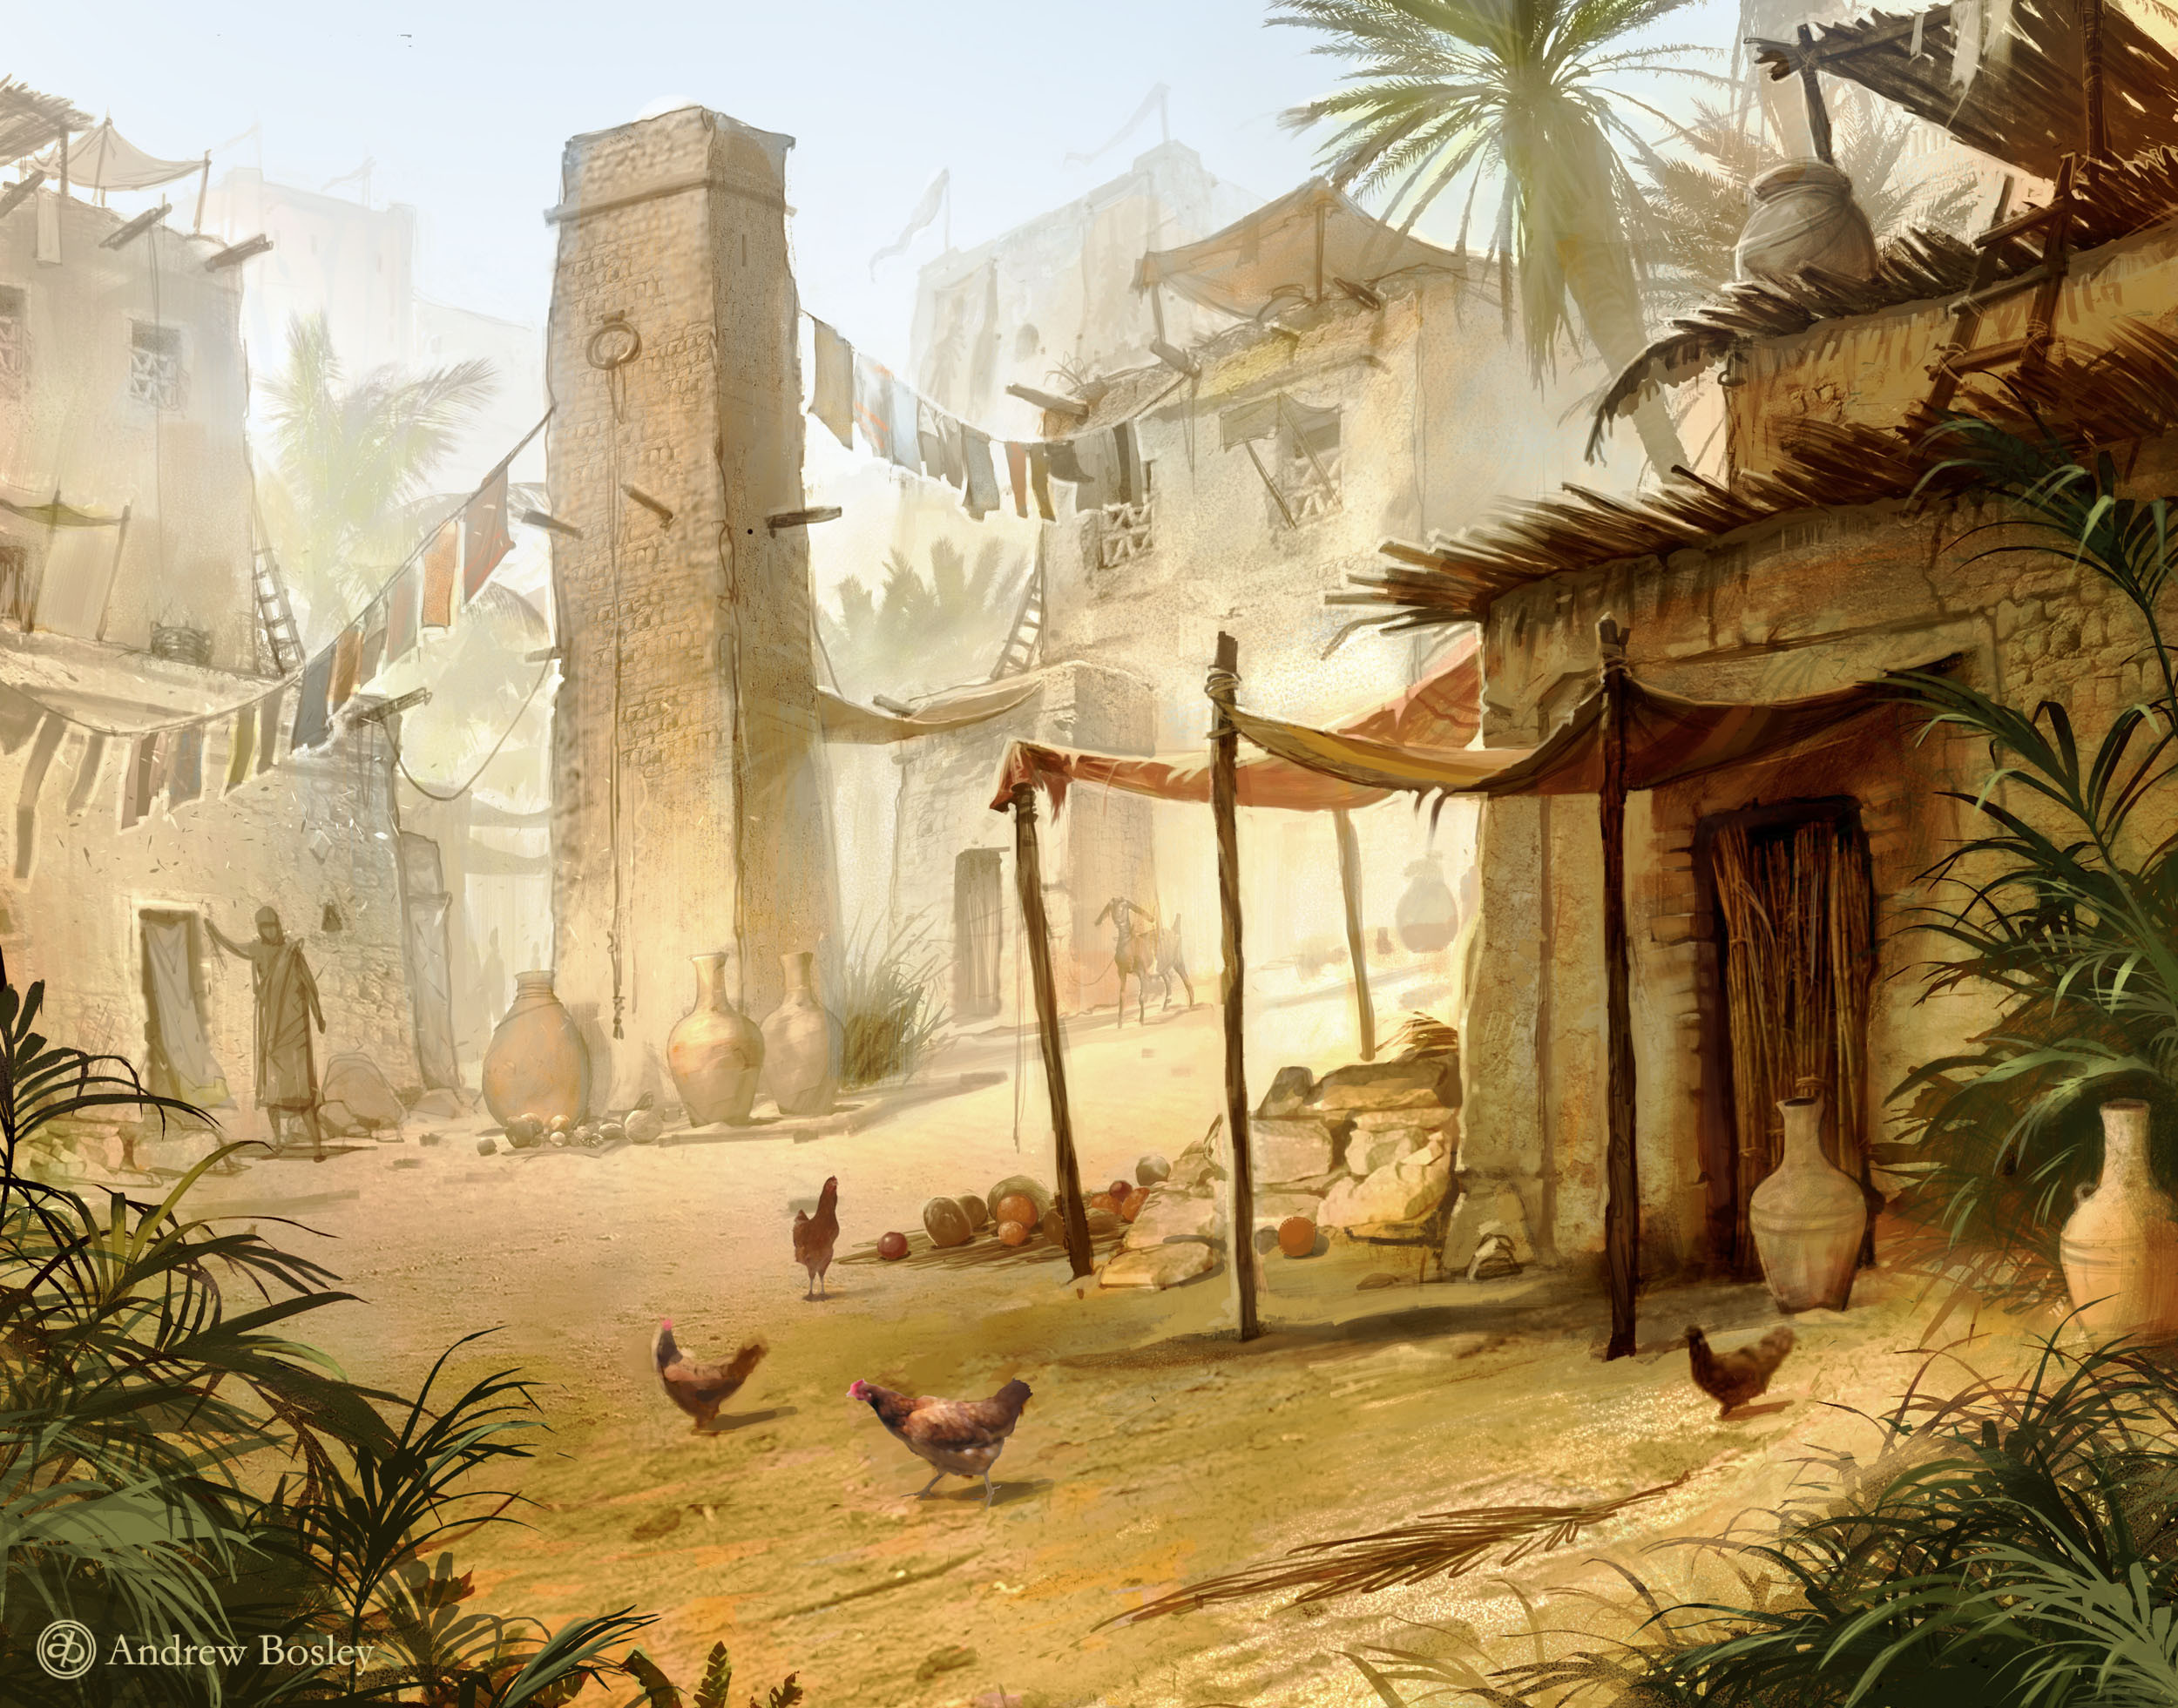
\includegraphics[width=0.7\linewidth]{images/village.jpg}
\end{figure}

\epigraph{\textit{
"I live in a world of fire and sand. The crimson sun scorches the life from
 anything that crawls or flies, and storms of sand scour the foliage from
 the barren ground. This is a land of blood and dust, where tribes of feral
 elves sweep out of the salt plains to plunder lonely caravans, mysterious
 singing winds call travelers to slow suffocation in the Sea of Silt, and
 selfish kings squander their subjects’ lives building gaudy palaces and
 garish tombs. This bleak wasteland is Athas, and it is my home." } } { - The Wanderer’s Journal }

\textit{I've compiled a few lists of things that most characters would know to use as a player handout in my games.
During character creation, hand out each section that applies to each character (race, social class, city state)
as they are chosen, the others that don't get used can be quick reference guides for things like knowledge checks,
or info for when players interact with NPCs and are asking questions.}

\section{General}
\begin{description}
    \item There are no gods
    \item A full skin or pot of water is worth your life
    \item You can’t trust an Elf
    \item Athas is an endless wasteland, spotted by tiny oases, and filled with predators
    \item The desolate condition of Athas is the result of unchecked magic use
    \item Arcane spellcasters are mistrusted at best, and reviled more often than not
    \item The tablelands are dotted with ruins from an ancient past
    \item Every creature, and even a few plants have some form of latent psionic power
    \item There are seven city states: Balic, Draj, Gulg, Nibenay, Raam, Tyr, and Urik, each ruled by an oppressive Sorcerer King
    \item Even more powerful than the Sorcerer Kings is The Dragon, who demands tribute of 1000 slaves from each city state each year
\end{description}

\subsection{Races}
\subsection{Dwarves}

\begin{description}
    \item Nothing comes before family except your Focus
    \item A Dwarf’s chief love is toil
    \item If a Dwarf dies with his Focus incomplete, he returns as an undead Banshee to haunt the objective of his Focus
    \item Dwarves are hairless and consider the very idea of hair repulsive, though carvings at the Dwarven city of Kled show Dwarves sporting hair and beards in the ancient past
    \item The three primary Dwarven settlements are North and South Ledopolus, and Kled, a Dwarven village near the City State of Tyr
    \item The Dwarves of North and South Ledopolis are trying to build a bridge to connect the two villages, but the giants living on Ledo Island in the center keep wading out across the Silt Sea to destroy the bridge
    \item Dwarves shun arcane magic as a rule, and while they will travel with a spellcaster who proves themselves a worthy companion (by actively working towards the Dwarf’s Focus), they rarely ever fully trust a wizard
    \item Dwarves who study The Way tend to excel in its use, and many Dwarves become Clerics of Earth, while Fire and Water also tend to attract Dwarven devotees.
    \item Dwarves almost always have a serious, sober demeanor. Only when they’ve completed their Focus do they allow other Dwarves, and their most trusted non-Dwarven friends see their joy and sense of humor (and that lasts only until another Focus is chosen)
    \item Nothing is impossible in the eyes of a Dwarf. The fastest way to earn the enmity of a Dwarf is to tell him “It can’t be done.”
\end{description}

\subsection{Elves}

\begin{description}
    \item \textit{"Death is stillness, so run, you Elves. Dance to the beat of life, for the moment is quick and oh so short. There is nothing as fast nor as proud nor as wonderfully made as an Elf."}
    \item You can’t trust anyone, especially outside your own tribe (until they’ve passed a series of trust tests)
    \item Those that fall behind are left behind
    \item To ride rather than run is to have no honor
    \item Of all the races, Elves are the most likely practitioners of sorcery, particularly Defiler magic
    \item Elves do not usually excel in the pursuit of Psionics, because most lack the dedication to continue their studies.
    \item Elves live for the “now”. They have little care for anything but instant gratification. Looking back the past reminds them of lost opportunities for fleeting happiness, while the future is almost certainly going to be worse than now.
    \item Elves revere Coraanu Star Racer, the Warrior Thief and mythical “first elf” as a pinnacle of Elvishness to aspire to.
    \item Elves will often flaunt a stolen item right in front of its former owner. Elven culture dictates the victim should congratulate the Elf on the possession of such an attractive item. Those who do not are considered poor sports.
    \item Elven chiefs are customarily given a percentage of the gains from any raid. An Elf who holds out on his chief is considered disloyal to his tribe.
\end{description}

\subsection{Halflings}

\begin{description}
    \item Death is preferable to slavery
    \item Wages are a form of slavery
    \item Halfling speech is riddled with idioms and cultural references
    \item Halflings have a very rich and diverse culture
    \item Halflings are more concerned with how their deeds help improve Halfling culture, rather than amassing great treasures
    \item Halflings are mainly carnivorous and prefer their meat raw
    \item Halflings are very concerned with the condition of the environment and will take any measure to keep their jungle from becoming like the rest of the tablelands
    \item Halflings have little to no concept of conquest and plunder in their culture
    \item Halflings don’t require as much food or water as the larger races
    \item Halfling chiefs are much like the Sorcerer Kings of the great city states, but are all Preservers rather than Defilers
\end{description}

\subsection{Half-Elves}

\begin{description}
    \item Half-Elves pride themselves on their self-reliance
    \item Most Half-Elven children are usually abandoned by their Elven parent
    \item Half-Elves almost always have human names, most being unable to earn a proper Elven name.
    \item Half-Elves predominantly live within human society, or out in the wilderness as hermits as they have no separate culture of their own
    \item Half-Elves readily take to studies and professions that favor solitary independence. Magic, Psionics, and the element of Water all are common pursuits.
    \item Half-Elves also become Druids quite often due to their natural inclination towards solitude
    \item Half-Elves often find the Templarate a fitting life.
    \item Many Half-Elves resent Elves, yet also feel a need to win their approval
    \item A Half-Elf is just as likely to seek companionship from an animal as they are from another person
    \item Due to their heightened senses and the fact that they are usually more reliable than Elves, many Half-Elves are hired by merchant caravans as scouts and outriders
\end{description}

\subsection{Half-Giants}

\begin{description}
    \item You have no culture/cultural identity of your own, so you readily adopt the culture and behavior of those you admire
    \item Despite their size and fearsome reputation, Half-Giants tend to possess an almost child like friendliness and curiosity
    \item Half-Giants also have a ferocious temper, only a fool would tempt a Half-Giant’s rage
    \item Half-Giants rarely have the patience or mental facilities for learning magic or psionics, though the occasional clever Half-Giant might dabble with Metacreativity or Psychokinesis and become a truly terrifying psychic warrior
    \item Half-Giants rarely become leaders, more often than not they follow an admired or charismatic friend into adventure, or whomever they find particularly interesting
    \item Half-Giants require twice as much food and water as other demihumans
    \item Your large size sometimes causes you to accidentally break human-sized dwellings and furniture
    \item Most Half-Giants live their lives as slave soldiers, though the more ambitious and adventurous among them sell their services as highly sought after mercenaries
    \item If you meet someone interesting enough, you might completely abandon whatever it is you’re doing to follow them
    \item Legend has it a great Sorcerer King created your race long ago.
\end{description}

\subsection{Humans}

\begin{description}
    \item Humans are ubiquitous in the tablelands of Athas
    \item Humans are the most adaptable among races and fill stations from the lowliest slaves and hermits to the rulers of the great trading houses and high templars of the Sorcerer Kings themselves.
    \item Humans take readily to studying The Way, as well as the worship of the elements.
    \item Most humans distrust and fear arcane magic. Many wizards, both preservers and defilers, have been killed by an angry mob.
    \item There is nothing human ingenuity cannot accomplish.
\end{description}

\subsection{Muls}

\begin{description}
    \item You were born a slave, and you will likely die a slave
    \item Most Muls are kept as gladiator slaves, due to their nearly unmatched physical prowess
    \item The life of a gladiatorial slave can be almost as lavish as that of the nobility, if you continue to perform well
    \item While many Muls have the opportunity to win their freedom many choose to remain in the arenas
    \item You are stronger than the other races, what would be considered intolerably painful for others is only a mere distraction for you
    \item Your stamina is unparallelled. You can quarry rock for a full 12 hours with no rest or walk for days without stopping. As long as you sleep at least 6 hours every few days, you don’t suffer from fatigue.
    \item Unlike the Dwarves they are descended from, Muls often sport tattoos, from shoulder markings denoting victory in the arenas to full body tattoos.
    \item Most Mul births result in the death of the mother, especially if the mother is human.
    \item Muls are born sterile and can have no children.
    \item Despite their formidable physique Muls don’t always make good soldiers. They’re smart enough to tell when a commander is making a tactical error, and stubborn enough to refuse such orders.
\end{description}

\subsection{Thri-kreens}

\begin{description}
    \item Elves are tasty
    \item Humanoid customs are strange, and most of the time none of the other races seem to understand Thri-kreen ways.
    \item Thri-kreen have a pack mentality, and tend to view everything from a predator/prey point of view.
    \item Many Thri-kreen develop psionic powers beyond a simple wild talent, they make excellent Monks and Psionicists
    \item Some Thri-kreen are capable of delivering a poisonous bite
    \item Thri-kreen possess great agility and can leap great distances
    \item Since you do not sleep, you don’t understand why other races seem to become lazy during certain parts of the day
    \item You live for the hunt, little else interests you
    \item Thri-kreen have no disposition towards magic, especially arcane
    \item There are no known Thri-kreen settlements within the tablelands
\end{description}

\section{Caste}
\subsection{Freeman}

\begin{description}
    \item Templars can enter your home at will
    \item While you are not a slave, you must devote most of your time to earning enough money to keep your freedom
    \item Most freemen are crafters and artisans, others run market stalls or smaller businesses like taverns and brothels in the less savory parts of the city
    \item Most freemen own at least a small home
    \item Very occasionally a freeman is successful (or lucky) enough to rise into the ranks of nobility through sheer wealth
\end{description}

\subsection{Noble}

\begin{description}
    \item You have been born into a life of luxury, but also one of political intrigue
    \item You never set foot outside of the safety of your villa or compound without your guards, palanquin to ride in, or at the very least a good disguise.
    \item You have slaves to deal with the things lesser people have to do themselves
    \item Many nobles have personal bards, consorts, and other “toys” to keep them occupied.
    \item A favorite pastime of the nobility is betting on their favorite gladiator(s)
\end{description}

\subsection{Slave (Artist)}

\begin{description}
    \item You are a slave. You were either born into slavery, could not pay a debt, or were caught committing a crime and were sold into slavery.
    \item Your owner/master may have taught you how to read and write, but this skill is illegal in all of the city states, and will likely get you killed if anyone finds out
    \item The best way to stay alive is by creating whatever type of art keeps your master happy
    \item You live a lavish lifestyle for a slave, rivaled only by gladiatorial champions
    \item Attempted escape carries a penalty of death
\end{description}

\subsection{Slave (Farmer)}

\begin{description}
    \item You are a slave. You were either born into slavery, could not pay a debt, or were caught committing a crime and were sold into slavery.
    \item To earn your freedom, you have to work off your debt
    \item When you aren’t working you are sleeping, you have little time for anything else
    \item If you move your hand to your mouth without permission while working in the fields, you will lose a hand. If it happens again, you will be beaten to death.
    \item Attempted escape carries a penalty of death
\end{description}

\subsection{Slave (Gladiator)}

\begin{description}
    \item You are a slave. You were either born into slavery, could not pay a debt, or were caught committing a crime and were sold into slavery.
    \item Your purpose is to fight for the entertainment of others, sometimes to the death
    \item The life of a gladiatorial slave can be almost as lavish as that of the nobility, if you continue to perform well
    \item You can win/buy your freedom if you are good. If you aren’t, you will likely end up pitted against a superior opponent so that your death can entertain the crowds
    \item Attempted escape carries a penalty of death
\end{description}

\subsection{Slave (Laborer)}

\begin{description}
    \item You are a slave. You were either born into slavery, could not pay a debt, or were caught committing a crime and were sold into slavery.
    \item To earn your freedom, you have to work off your debt
    \item When you aren’t working you are sleeping, you have little time for anything else
    \item All you know of life is either toiling day in and day out in a mine or quarry, or building something for your master
    \item Attempted escape carries a penalty of death
\end{description}

\subsection{Slave (Soldier)}

\begin{description}
    \item You are a slave. You were either born into slavery, could not pay a debt, or were caught committing a crime and were sold into slavery.
    \item To earn your freedom, you have to work off your debt by completing your term of deployed service
    \item Attempted escape carries a penalty of death
    \item Most of your life is spent in the training yards, preparing for war
    \item When battle comes, you can be sure to be placed on the front lines where fighting is the fiercest and mortality rates are staggeringly high
\end{description}

\subsection{Tribal (can be used in place of both social standing, as well as city state)}

\begin{description}
    \item City states seem claustrophobic to you, everything is too close, there are too many people, and they stink of shit.
    \item Whether a tribe of nomadic herdsmen, hunter-gatherers, or raiders, you are often on the move, never staying put for too long.
    \item You have seen things out in the wastelands of Athas that most people in the cities couldn’t even comprehend.
    \item Most tribes, regardless of vocation, tend to be comprised of a single race. The exception to this, of course, are the tribes of escaped slaves.
    \item In most tribes the leader is the strongest individual, and changes in leadership tend to be violent.
\end{description}

\section{City States}
\subsection{Balic (based on ancient Greek and Roman culture)}

\begin{description}
    \item Andropinis claims he was elected to the position of lifelong dictator over 700 years ago
    \item Templars in Balic are elected for 10-year terms. Andropinis usually makes it clear which ones he favors, and on the rare occasion that the “wrong” one wins, they disappear
    \item Andropinis’ personal army consists of 10,000 mostly human foot soldiers carrying lances, large wooden shields, and bone daggers (hoplites)
    \item Every citizen of Balic is a member of the militia and spends every 10th month assisting the regular army patrol the fields to reduce crop and stock loss to Giants who regularly raid from across the Silt Sea
    \item Balic is situated in the Estuary of the Forked Tongue, a very defensible location as far as invasion from the other city-states is concerned, as it is surrounded by parts of the Silt Sea on the North, East, and South sides
    \item Balic has a strong economic district, which specializes in trade of olive oil, kank nectar, and pottery.
    \item The Agora, or market square is completely ringed in by the Elven market, making it impossible to do any legitimate business without dealing with the dubious offers of the Elven merchants
    \item The Silt Sea contains numerous islands inhabited by giants, and dotted with crumbling ruins.
    \item Shipfloaters are psionicists who telepathically levitate ships to traverse the Sea of Silt.
    \item \textbf{Rumour:} The Dwarves of North and South Ledopolis are trying to build a bridge to connect the two villages, but the giants living on Ledo Island in the center keep wading out across the Silt Sea to destroy the bridge
\end{description}

\subsection{Draj (based on Aztec culture)}

\begin{description}
    \item The Mighty and Omnipotent Tectuktitlay, Father of Life and Master of the Two Moons claims to be a living god
    \item Templars in Draj are known as Moon Priests
    \item The fertile soil surrounding Draj allows it to grow many crops, including grain for bread and hemp, which makes for good ropes
    \item Draj is almost constantly at war, raiding villages and even other city states for captives to be sacrificed on the steps of Tectuktitlay’s pyramid, overlooking the gladiatorial arena
    \item Knowledge of history is expressly forbidden by Tectuktitlay, nothing beyond mortal memory is really known about the past of this city
    \item Draji warriors decorate themselves with the skins of various beasts and animals, and carry obsidian-edged clubs called Macuahuitl as well as short harpoons
    \item Criminals in Draj receive only one sentence: death, either by execution or by caging (a very slow death by exposure).
    \item Crime, especially theft is so looked down upon by Draji culture that most citizens would rather sell themselves into slavery than steal.
    \item Instead of a wall, the entrance to the city state is surrounded by expansive mud flats, which provide plenty of protection from invaders.
    \item \textbf{Rumour:} Draj has vast storehouses of grains and hemp that it keeps hidden from everybody in order to drive up their prices when trading with other city states.
\end{description}

\subsection{Gulg (based on various African savannah cultures)}

\begin{description}
    \item Lalali-Puy, the oba, or forest goddess is the only ruler of a city state who enjoys the popular support of her people
    \item Gulg lies at the southern end of the Crescent Forest
    \item Nearly everything in Gulg is made from Agafari wood, even the houses are carved out of the very trees
    \item Lalali-Puy controls all economic activity within Gulg directly, taking all the food produced and distributing it amongst her people. Merchants from outside the city can trade with the city state, but it is forbidden to trade with the citizens themselves.
    \item Citizens of Gulg also have the right to appeal directly to Lalai-Pui for an audience if they need a matter resolved.
    \item Gulg’s city wall is a magically infused hedge of thorny brambles that actively seek out the flesh of those who try to penetrate it.
    \item Despite what the title of city state invokes, Gulg is actually a collection of villages all crammed together within the shelter of the city wall
    \item When a new Nganga (templar) is chosen, the district they come from holds a funeral service to symbolize that the citizen they once were is no more.
    \item The templars of Gulg wear masks or face paint to hide their features and strike fear into those who would oppose the Oba
    \item \textbf{Rumour:} If not for the power of the Oba and her Judagas (warriors), Nibenay would likely have destroyed or taken Gulg over long ago.
\end{description}

\subsection{Nibenay (based on Angkor culture)}

\begin{description}
    \item Nobody can remember the last time Nibenay, the Shadow King was seen outside the Naggaramakam
    \item The Naggaramakam is a walled central district in which only Nibenay’s Templars may enter and leave. Slaves who enter here are never permitted to leave again
    \item Nibenay lies at the northern end of the Crescent Forest
    \item Every surface of every building in Nibenay is covered with carvings of various figures
    \item Nibenay holds the only permanent Elven market, which is run by the Sky Singers tribe
    \item The Monastery of the Exalted Path is an all male psionics academy, the female counterpart is called The Monastery of Serene Bliss. Both are well respected
    \item A line of large statues of King Nibenay stand on each side of the main road to the city. The statues are called the Omnipotent Receivers as it is believed that the Shadow King can see through their eyes.
    \item Some people believe that the Shadow King hasn’t been seen because he actually died a long time ago.
    \item All Nibenese templars are female and are sometimes referred to as Nibenay’s Wives
    \item \textbf{Rumour:} the ruins of Giustenal are said to contain a powerful psionic entity
\end{description}

\subsection{Raam (based on ancient Indian and Egyptian culture)}

\begin{description}
    \item The Great Vizier Abalach-Re claims to be the emissary of a higher power known as Badna
    \item Abalach-Re assures citizens that Badna watches her closely and will strike her down if she falters in her duties, but few believe her.
    \item Almost no citizens of Raam actually respect their Sorcerer Queen, and there is open talk of rebellion in the streets
    \item The nobles of Raam are little more than warlords constantly fighting against each other and jockeying for position in the inevitable revolution
    \item Templars of Raam almost never travel alone, lest they are murdered in the streets
    \item Raam culture consists of a rigid caste system
    \item While it was once an economic powerhouse, and still remains the largest city-state on the tablelands, Raam’s infrastructure has fallen almost completely apart due to the indifference of Abalach-Re who prefers to take pleasure in whatever strikes her fancy rather than rule her city.
    \item Crime runs rampant in the streets without the presence of templars to maintain order.
    \item Abalach-Re has born hundreds of illegitemate children over the 30 or so generations that she has ruled Raam. Known as the Offspring, many of her children have exhibited unusual psionic and arcane talents.
    \item \textbf{Rumour:} Stay away from the ruins of Yaramuke. Hamanu of Urik used such foul magics to destroy it that the entire area, including the fresh water springs that flow from within are all posionous
\end{description}

\subsection{Tyr (based on the culture of Tyre)}

\begin{description}
    \item King Kalak, the Tyrant of Tyr has allocated an inordinate number of slaves towards working to build his ziggurat, including those owned by the nobility
    \item Even the iron mines, upon which Tyr’s economy is based have been shut down to allocate more resources to the ziggurat
    \item Nobody knows what the ziggurat is for
    \item Kalak’s Templars as well as his personal guard are all armed with iron swords
    \item As in most of the city states, while Tyr’s Elven Market is always in the same area, the vendors are always changing from one day to the next.
    \item Because most of the slave laborers have been working on the ziggurat, the remaining gladiatorial slaves have been putting on more and more impressive fights, rather than the barbarically uneven matches that were normally seen before. This in turn is increasing the draw that the games have to the point where seat prices have risen dramatically.
    \item People are starting to whisper that King Kalak has gone mad.
    \item Tyr is located in a valley along the edge of the Ringing Mountains
    \item Taxes have also risen dramatically since Kalak began the construction of his ziggurat.
    \item \textbf{Rumour:} Tyr was built atop the ruined foundations of an ancient city. Though many of the passages and byways are blocked off either by more recent construction, or shifting dunes, there are still many hidden access points to various locations under the city. This area is known as UnderTyr.
\end{description}

\subsection{Urik (based on Babylonian culture)}

\begin{description}
    \item King Hamanu trains daily with his warriors, even the slaves
    \item The walls of Urik are famous for being nearly unbreachable
    \item You would do well to remember all of Hamanu’s many laws if you don’t want to find yourself being sold into slavery by a templar
    \item Urik lies near the Dragon’s Bowl - a massive crater with 1000 foot high cliffs leading down to a large lake in the bottom.
    \item The majority of the tools and weapons found in Urik are made from obsidian, which is mined from the nearby Smoking Crown mountains.
    \item Statues of lions top the massive walls, where guards patrol with their bows and obsidian-tipped arrows
    \item Urik’s gladiatorial arena, known as the Pit of Black Death, rests in an old abandoned obsidian mine, its walls lined with razor sharp obsidian.
    \item Children are tested by templars at an early age and are assigned a vocation based on their abilities. It is extremely rare for a change in career in Urik.
    \item Children who show talent in The Way are taken from their parents and sent to Hamanu’s school of the mind for training.
    \item \textbf{Rumour:} King Kalak of Tyr has stopped production of iron, Hamanu might send his army to get more iron!
\end{description}
